\documentclass{report}
\usepackage{pdfpages}
\usepackage{listings}
\usepackage{color}
\usepackage{amssymb}
\usepackage{amsmath}
\usepackage{centernot}
\usepackage{scalerel}
\usepackage{varwidth}
\usepackage{xcolor}
\usepackage{graphicx}
%\usepackage[margin=0.5in]{geometry}
\usepackage[top=1in,bottom=1in]{geometry}
\usepackage[utf8]{inputenc}

\usepackage{circuitikz}
\usepackage{tkz-graph}
\usepackage{tikz}
\usetikzlibrary{matrix,calc,arrows,arrows.meta,shapes,positioning,chains}


%%% BEGIN lst configs for VHDL
    \definecolor{mygreen}{rgb}{0,0.6,0}
    \definecolor{mygray}{rgb}{0.5,0.5,0.5}
    \definecolor{mymauve}{rgb}{0.58,0,0.82}

    \lstset{ %
      backgroundcolor=\color{white},   % choose the background color; you must add \usepackage{color} or \usepackage{xcolor}; should come as last argument
      basicstyle=\ttfamily,        % the size of the fonts that are used for the code
      breakatwhitespace=false,         % sets if automatic breaks should only happen at whitespace
      breaklines=true,                 % sets automatic line breaking
      captionpos=b,                    % sets the caption-position to bottom
      commentstyle=\color{mygreen},    % comment style
      deletekeywords={...},            % if you want to delete keywords from the given language
      escapeinside={\%*}{*)},          % if you want to add LaTeX within your code
      extendedchars=true,              % lets you use non-ASCII characters; for 8-bits encodings only, does not work with UTF-8
      frame=single,	                   % adds a frame around the code
      keepspaces=true,                 % keeps spaces in text, useful for keeping indentation of code (possibly needs columns=flexible)
      keywordstyle=\color{blue},       % keyword style
      language=VHDL,                 % the language of the code
      morekeywords={*,...},           % if you want to add more keywords to the set
      rulecolor=\color{black},         % if not set, the frame-color may be changed on line-breaks within not-black text (e.g. comments (green here))
      showspaces=false,                % show spaces everywhere adding particular underscores; it overrides 'showstringspaces'
      showstringspaces=false,          % underline spaces within strings only
      showtabs=false,                  % show tabs within strings adding particular underscores
      stringstyle=\color{mymauve},     % string literal style
      tabsize=2,	                   % sets default tabsize to 2 spaces
      title=\lstname                   % show the filename of files included with \lstinputlisting; also try caption instead of title
    }
%%% END lst configs for VHDL

\newcommand\showdiv[1]{\overline{\smash{\hstretch{.5}{)}\mkern-3.2mu\hstretch{.5}{)}}#1}}
\newcommand\ph[1]{\textcolor{white}{#1}}


\makeatletter
% we use \prefix@<level> only if it is defined
\renewcommand{\@seccntformat}[1]{%
  \ifcsname prefix@#1\endcsname
    \csname prefix@#1\endcsname
  \else
    \csname the#1\endcsname\quad
  \fi}
% define \prefix@section
\newcommand\prefix@section{}
\newcommand\prefix@subsection{}
\makeatother


%%% BEGIN Karnaugh map code
    %isolated term
    %#1 - Optional. Space between node and grouping line. Default=0
    %#2 - node
    %#3 - filling color
    \newcommand{\implicantsol}[3][0]{
        \draw[rounded corners=3pt, fill=#3, opacity=0.3] ($(#2.north west)+(135:#1)$) rectangle ($(#2.south east)+(-45:#1)$);
        }


    %internal group
    %#1 - Optional. Space between node and grouping line. Default=0
    %#2 - top left node
    %#3 - bottom right node
    %#4 - filling color
    \newcommand{\implicant}[4][0]{
        \draw[rounded corners=3pt, fill=#4, opacity=0.3] ($(#2.north west)+(135:#1)$) rectangle ($(#3.south east)+(-45:#1)$);
        }

    %group lateral borders
    %#1 - Optional. Space between node and grouping line. Default=0
    %#2 - top left node
    %#3 - bottom right node
    %#4 - filling color
    \newcommand{\implicantcostats}[4][0]{
        \draw[rounded corners=3pt, fill=#4, opacity=0.3] ($(rf.east |- #2.north)+(90:#1)$)-| ($(#2.east)+(0:#1)$) |- ($(rf.east |- #3.south)+(-90:#1)$);
        \draw[rounded corners=3pt, fill=#4, opacity=0.3] ($(cf.west |- #2.north)+(90:#1)$) -| ($(#3.west)+(180:#1)$) |- ($(cf.west |- #3.south)+(-90:#1)$);
    }

    %group top-bottom borders
    %#1 - Optional. Space between node and grouping line. Default=0
    %#2 - top left node
    %#3 - bottom right node
    %#4 - filling color
    \newcommand{\implicantdaltbaix}[4][0]{
        \draw[rounded corners=3pt, fill=#4, opacity=0.3] ($(cf.south -| #2.west)+(180:#1)$) |- ($(#2.south)+(-90:#1)$) -| ($(cf.south -| #3.east)+(0:#1)$);
        \draw[rounded corners=3pt, fill=#4, opacity=0.3] ($(rf.north -| #2.west)+(180:#1)$) |- ($(#3.north)+(90:#1)$) -| ($(rf.north -| #3.east)+(0:#1)$);
    }

    %group corners
    %#1 - Optional. Space between node and grouping line. Default=0
    %#2 - filling color
    \newcommand{\implicantcantons}[2][0]{
        \draw[rounded corners=3pt, opacity=.3] ($(rf.east |- 0.south)+(-90:#1)$) -| ($(0.east |- cf.south)+(0:#1)$);
        \draw[rounded corners=3pt, opacity=.3] ($(rf.east |- 8.north)+(90:#1)$) -| ($(8.east |- rf.north)+(0:#1)$);
        \draw[rounded corners=3pt, opacity=.3] ($(cf.west |- 2.south)+(-90:#1)$) -| ($(2.west |- cf.south)+(180:#1)$);
        \draw[rounded corners=3pt, opacity=.3] ($(cf.west |- 10.north)+(90:#1)$) -| ($(10.west |- rf.north)+(180:#1)$);
        \fill[rounded corners=3pt, fill=#2, opacity=.3] ($(rf.east |- 0.south)+(-90:#1)$) -|  ($(0.east |- cf.south)+(0:#1)$) [sharp corners] ($(rf.east |- 0.south)+(-90:#1)$) |-  ($(0.east |- cf.south)+(0:#1)$) ;
        \fill[rounded corners=3pt, fill=#2, opacity=.3] ($(rf.east |- 8.north)+(90:#1)$) -| ($(8.east |- rf.north)+(0:#1)$) [sharp corners] ($(rf.east |- 8.north)+(90:#1)$) |- ($(8.east |- rf.north)+(0:#1)$) ;
        \fill[rounded corners=3pt, fill=#2, opacity=.3] ($(cf.west |- 2.south)+(-90:#1)$) -| ($(2.west |- cf.south)+(180:#1)$) [sharp corners]($(cf.west |- 2.south)+(-90:#1)$) |- ($(2.west |- cf.south)+(180:#1)$) ;
        \fill[rounded corners=3pt, fill=#2, opacity=.3] ($(cf.west |- 10.north)+(90:#1)$) -| ($(10.west |- rf.north)+(180:#1)$) [sharp corners] ($(cf.west |- 10.north)+(90:#1)$) |- ($(10.west |- rf.north)+(180:#1)$) ;
    }

    %Empty Karnaugh map 4x4
    \newenvironment{Karnaugh}%
    {
    \begin{tikzpicture}[baseline=(current bounding box.north),scale=0.8]
    \draw (0,0) grid (4,4);
    \draw (0,4) -- node [pos=0.7,above right,anchor=south west] {de} node [pos=0.7,below left,anchor=north east] {bc} ++(135:1);
    %
    \matrix (mapa) [matrix of nodes,
            column sep={0.8cm,between origins},
            row sep={0.8cm,between origins},
            every node/.style={minimum size=0.3mm},
            anchor=8.center,
            ampersand replacement=\&] at (0.5,0.5)
    {
                           \& |(c00)| 00         \& |(c01)| 01         \& |(c11)| 11         \& |(c10)| 10         \& |(cf)| \phantom{00} \\
    |(r00)| 00             \& |(0)|  \phantom{0} \& |(1)|  \phantom{0} \& |(3)|  \phantom{0} \& |(2)|  \phantom{0} \&                     \\
    |(r01)| 01             \& |(4)|  \phantom{0} \& |(5)|  \phantom{0} \& |(7)|  \phantom{0} \& |(6)|  \phantom{0} \&                     \\
    |(r11)| 11             \& |(12)| \phantom{0} \& |(13)| \phantom{0} \& |(15)| \phantom{0} \& |(14)| \phantom{0} \&                     \\
    |(r10)| 10             \& |(8)|  \phantom{0} \& |(9)|  \phantom{0} \& |(11)| \phantom{0} \& |(10)| \phantom{0} \&                     \\
    |(rf) | \phantom{00}   \&                    \&                    \&                    \&                    \&                     \\
    };
    }%
    {
    \end{tikzpicture}
    }

    % K map q2q3\Xq1
    \newenvironment{KarnaughG}%
    {
    \begin{tikzpicture}[baseline=(current bounding box.north),scale=0.8]
    \draw (0,0) grid (4,4);
    \draw (0,4) -- node [pos=0.9,above right,anchor=south west] {$XQ_1$} node [pos=0.9,below left,anchor=north east] {$Q_2Q_3$} ++(135:1);
    %
    \matrix (mapa) [matrix of nodes,
            column sep={0.8cm,between origins},
            row sep={0.8cm,between origins},
            every node/.style={minimum size=0.3mm},
            anchor=8.center,
            ampersand replacement=\&] at (0.5,0.5)
    {
                           \& |(c00)| 00         \& |(c01)| 01         \& |(c11)| 11         \& |(c10)| 10         \& |(cf)| \phantom{00} \\
    |(r00)| 00             \& |(0)|  \phantom{0} \& |(1)|  \phantom{0} \& |(3)|  \phantom{0} \& |(2)|  \phantom{0} \&                     \\
    |(r01)| 01             \& |(4)|  \phantom{0} \& |(5)|  \phantom{0} \& |(7)|  \phantom{0} \& |(6)|  \phantom{0} \&                     \\
    |(r11)| 11             \& |(12)| \phantom{0} \& |(13)| \phantom{0} \& |(15)| \phantom{0} \& |(14)| \phantom{0} \&                     \\
    |(r10)| 10             \& |(8)|  \phantom{0} \& |(9)|  \phantom{0} \& |(11)| \phantom{0} \& |(10)| \phantom{0} \&                     \\
    |(rf) | \phantom{00}   \&                    \&                    \&                    \&                    \&                     \\
    };
    }%
    {
    \end{tikzpicture}
    }

    %Empty Karnaugh map 2x4
    \newenvironment{Karnaughvuit}%
    {
    \begin{tikzpicture}[baseline=(current bounding box.north),scale=0.8]
    \draw (0,0) grid (4,2);
    \draw (0,2) -- node [pos=0.7,above right,anchor=south west] {bc} node [pos=0.7,below left,anchor=north east] {a} ++(135:1);
    %
    \matrix (mapa) [matrix of nodes,
            column sep={0.8cm,between origins},
            row sep={0.8cm,between origins},
            every node/.style={minimum size=0.3mm},
            anchor=4.center,
            ampersand replacement=\&] at (0.5,0.5)
    {
                          \& |(c00)| 00         \& |(c01)| 01         \& |(c11)| 11         \& |(c10)| 10         \& |(cf)| \phantom{00} \\
    |(r00)| 0             \& |(0)|  \phantom{0} \& |(1)|  \phantom{0} \& |(3)|  \phantom{0} \& |(2)|  \phantom{0} \&                     \\
    |(r01)| 1             \& |(4)|  \phantom{0} \& |(5)|  \phantom{0} \& |(7)|  \phantom{0} \& |(6)|  \phantom{0} \&                     \\
    |(rf) | \phantom{00}  \&                    \&                    \&                    \&                    \&                     \\
    };
    }%
    {
    \end{tikzpicture}
    }

    %Empty Karnaugh map 2x2
    \newenvironment{Karnaughquatre}%
    {
    \begin{tikzpicture}[baseline=(current bounding box.north),scale=0.8]
    \draw (0,0) grid (2,2);
    \draw (0,2) -- node [pos=0.7,above right,anchor=south west] {b} node [pos=0.7,below left,anchor=north east] {a} ++(135:1);
    %
    \matrix (mapa) [matrix of nodes,
            column sep={0.8cm,between origins},
            row sep={0.8cm,between origins},
            every node/.style={minimum size=0.3mm},
            anchor=2.center,
            ampersand replacement=\&] at (0.5,0.5)
    {
              \& |(c00)| 0          \& |(c01)| 1  \\
    |(r00)| 0 \& |(0)|  \phantom{0} \& |(1)|  \phantom{0} \\
    |(r01)| 1 \& |(2)|  \phantom{0} \& |(3)|  \phantom{0} \\
    };
    }%
    {
    \end{tikzpicture}
    }

    %Defines 8 or 16 values (0,1,X)
    \newcommand{\contingut}[1]{%
    \foreach \x [count=\xi from 0]  in {#1}
         \path (\xi) node {\x};
    }

    %Places 1 in listed positions
    \newcommand{\minterms}[1]{%
        \foreach \x in {#1}
            \path (\x) node {1};
    }

    %Places 0 in listed positions
    \newcommand{\maxterms}[1]{%
        \foreach \x in {#1}
            \path (\x) node {0};
    }

    %Places X in listed positions
    \newcommand{\indeterminats}[1]{%
        \foreach \x in {#1}
            \path (\x) node {X};
    }
%%% END Karnaugh map code


\begin{document}

\begin{titlepage}
    \centering
    {\scshape\LARGE University of Texas at Austin\par}
    \vspace{1cm}
    {\scshape\Large Digital Logic Design\par}
    \vspace{1.5cm}
    {\huge\bfseries Lab 7: VHDL for System Design\par}
    \vspace{2cm}
    {\Large\itshape Joshua Dong\par}
    jid295
    \vfill
    \today\par
    \vfill
    {\bfseries Contents\par}
    \vspace{0.5cm}
    \begin{varwidth}{\textwidth}
        \begin{enumerate}  
        \item Block Diagram
        \item State Graph
        \item VHDL Code
        \item Waveforms
        \item HDL Synthesis Report
        \item XDC File
        \end{enumerate}
    \end{varwidth}
    \vfill
\end{titlepage}


\subsection{Problem Statement}
Design an arithmetic unit that computes W = X*Y + Z, where {\bfseries X is 5
bits, Y is 3 bits and Z is 3 bits.} Assume that the start signal (St) is 1
exactly for one clock cycle.  When St is '1', in the first clock cycle, the
Multiplier (X) should be loaded from the bus. In the second clock cycle, the
Multiplicand (Y) should be loaded from the same bus. Finally, in the third
clock cycle, Z (the term to be added) should be loaded. Then the state machine
should multiply X by Y. Use a 9-bit accumulator, and design the multiplier
without using a counter. Use the overloaded addition operator to add. Use a
second adder to add Z to X*Y and store the result in the accumulator using a
fourth load signal.


\subsection{Block Diagram}
The following block diagram of the system shows registers, adders, MUXes, and
other components. Specified are the used signals, size of registers, adders,
etc. The design includes an active-high asynchronous RESET for your design.

%%% BEGIN tikz styles
    \tikzstyle{invis}  = [draw=white]
    \tikzstyle{block}  = [rectangle, draw, text width=4cm, text centered, minimum height=1em]
    \tikzstyle{block3} = [rectangle, draw, text width=12cm, text centered, minimum height=1em]
%%% END styles
\vspace{0.6cm}
%\vspace{-1cm}
\begin{tikzpicture}[node distance=2cm,scale=0.8]
    %% Nodes
    \node (ctrl) [block] {Control};
    \node (clk) [invis,right of=ctrl,right=1cm] {Clk};
    \node (acc) [block3,below of=ctrl,right=-2cm] {9-bit Accumulator (0000$|$X)};
    \node (adderY) [block,below of=acc,left=2cm] {3-bit Adder (Y)};
    \node (adderZ) [block,below of=acc,right=2cm] {3-bit Adder (Z)};

    %% Flows
    % Clk
    \draw [->] (clk) -- (ctrl);
    \draw [->] (clk) -| (acc);

    % Control
    \draw [<-] (ctrl) ++(2.25cm,1em) -- node[right] {$M$}
    ++(0cm,1.0cm) --
    ++(11cm,0cm) |-
    (acc.east);
    \draw [->] (ctrl) ++(.75cm,1em) -- node[right] {$Done$} ++(0cm,1cm);
    \draw [<-] (ctrl) ++(-.75cm,1em) -- node[right] {$St$} ++(0cm,1cm);
    \draw [<-] (ctrl) ++(-2.25cm,1em) -- node[right] {$Rst$} ++(0cm,1cm);

    \draw [->] (ctrl) ++(-1cm,-1em) -- node[right] {$Load$} ++(0cm,-1.7cm);
    \draw [->] (ctrl) ++(1cm,-1em) -- node[right] {$Shift$} ++(0cm,-1.7cm);

    \coordinate (Below y) at ($(adderY.south) + (0,-.8cm)$);
    \draw [->] (ctrl.west) ++(0,-0.3em) --
    ++(-.8cm,0) |-
    (Below y) -- node[right] {$Add1$}
    (adderY.south);
 
    \coordinate (Below z) at ($(adderZ.south) + (0,-1.6cm)$);
    \draw [->] (ctrl.west) ++(0,+0.3em) --
    ++(-1.6cm,0) |-
    (Below z) -- node[right] {$Add2$}
    (adderZ.south);

    % Acc
    \draw [->] (adderY.north) -- ++(0cm,1.7cm);
    \draw [->] (adderY.north) ++(-2cm,0cm) -- node[right] {$C_3$} ++(0cm,1.7cm);
    \draw [->] (adderZ.north) -- ++(0,1.7cm);
    \draw [->] (adderZ.north) ++(-2cm,0cm) -- node[right] {$C_3$} ++(0cm,1.7cm);
\end{tikzpicture}
\newpage
\subsection{State Graph}
Below is the state graph for the control circuit.

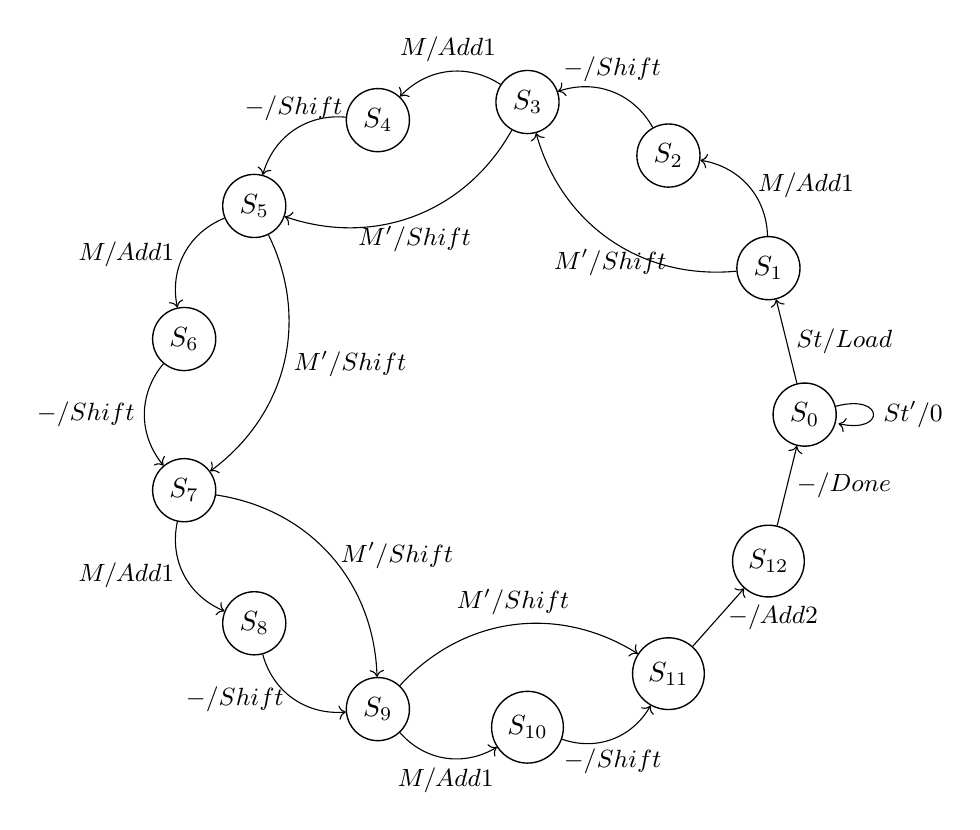
\begin{tikzpicture}
 \SetUpEdge[lw         = 1.0pt,
            color      = black,
            labelcolor = white]
  \GraphInit[vstyle=Normal] 
  \SetGraphUnit{3}
  \tikzset{VertexStyle/.append style={fill}}
    \Vertex[L={$S_0$},x=4.0,y=0.0]{0}
    \Vertex[L={$S_1$},x=3.54,y=1.86]{1}
    \Vertex[L={$S_2$},x=2.27,y=3.29]{2}
    \Vertex[L={$S_3$},x=0.48,y=3.97]{3}
    \Vertex[L={$S_4$},x=-1.42,y=3.74]{4}
    \Vertex[L={$S_5$},x=-2.99,y=2.65]{5}
    \Vertex[L={$S_6$},x=-3.88,y=0.96]{6}
    \Vertex[L={$S_7$},x=-3.88,y=-0.96]{7}
    \Vertex[L={$S_8$},x=-2.99,y=-2.65]{8}
    \Vertex[L={$S_9$},x=-1.42,y=-3.74]{9}
    \Vertex[L={$S_{10}$},x=0.48,y=-3.97]{10}
    \Vertex[L={$S_{11}$},x=2.27,y=-3.29]{11}
    \Vertex[L={$S_{12}$},x=3.54,y=-1.86]{12}

  % 0
  %\tikzset{EdgeStyle/.style={->,relative=true,in=30,out=-30,pos=5}}
  \path (0) edge [loop right] node {\small $St'/0$} (0);
  \path (0) edge [->,right] node {\small $St/Load$} (1);

  % bit 0
  \path (1) edge [->,right,relative=true,in=-140,out=-40] node {\small $M/Add1$} (2);
  \path (1) edge [->,below,relative=true,in=140,out=40] node {\small $M'/Shift$} (3);

  \path (2) edge [->,above,relative=true,in=-140,out=-40] node {\small $-/Shift$} (3);

  % bit 1
  \path (3) edge [->,above,relative=true,in=-140,out=-40] node {\small $M/Add1$} (4);
  \path (3) edge [->,below,relative=true,in=140,out=40] node {\small $M'/Shift$} (5);

  \path (4) edge [->,above,relative=true,in=-140,out=-40] node {\small $-/Shift$} (5);

  % bit 2
  \path (5) edge [->,left,relative=true,in=-140,out=-40] node {\small $M/Add1$} (6);
  \path (5) edge [->,right,relative=true,in=140,out=40] node {\small $M'/Shift$} (7);

  \path (6) edge [->,left,relative=true,in=-140,out=-40] node {\small $-/Shift$} (7);

  % bit 3
  \path (7) edge [->,left,relative=true,in=-140,out=-40] node {\small $M/Add1$} (8);
  \path (7) edge [->,right,relative=true,in=140,out=40] node {\small $M'/Shift$} (9);

  \path (8) edge [->,left,relative=true,in=-140,out=-40] node {\small $-/Shift$} (9);

  % bit 4
  \path (9) edge [->,below,relative=true,in=-140,out=-40] node {\small $M/Add1$} (10);
  \path (9) edge [->,above,relative=true,in=140,out=40] node {\small $M'/Shift$} (11);

  \path (10) edge [->,below,relative=true,in=-140,out=-40] node {\small $-/Shift$} (11);
    
  % add Z
  \path (11) edge [->,right] node {\small $-/Add2$} (12);

  % finish
  \path (12) edge [->,right] node {\small $-/Done$} (0);

  %\tikzset{EdgeStyle/.style={->,relative=true}}
  %  \Edge[label=$St/Load$](0)(1)

  %% 1
  %\Edge[label=$St/Load$](1)(2)
  %\Edge[label=$St/Load$](1)(3)

\end{tikzpicture}

\subsection{VHDL Code}
Below is simply an implementation of the state graph:
\lstinputlisting{ctrl.vhdl}

\subsection{Waveforms}
%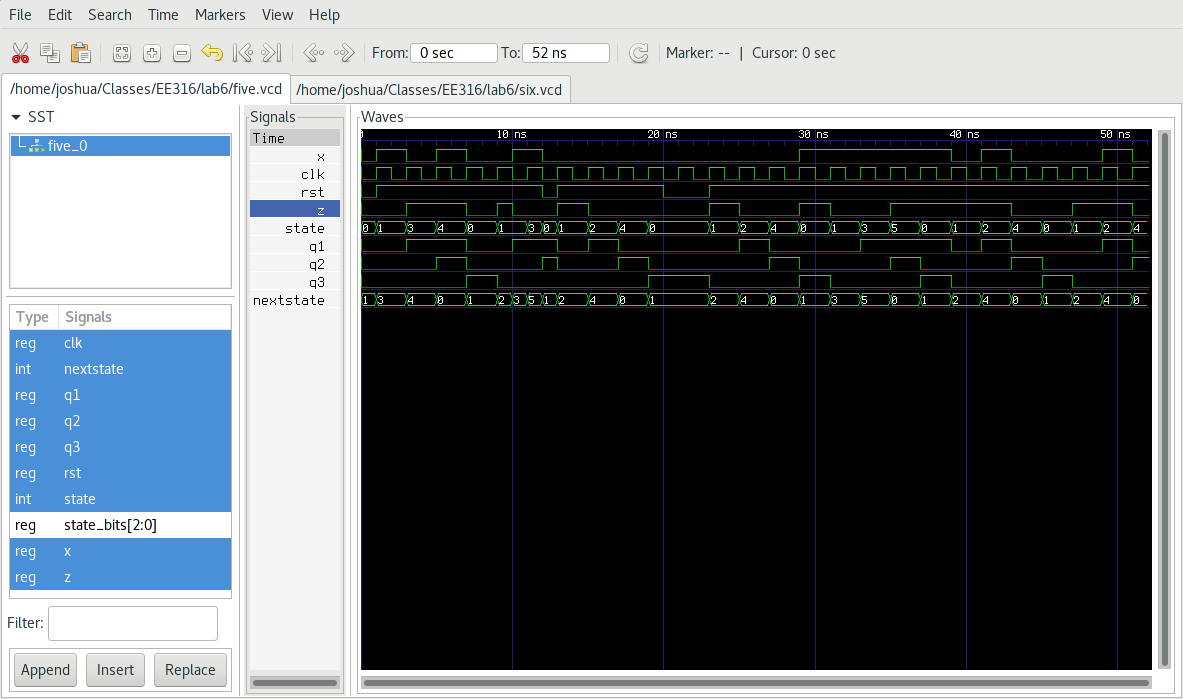
\includegraphics[width=\textwidth]{wave2}

\subsection{HDL Synthesis Report}
No latch was identified, so below is the HDL Synthesis Report page.


\subsection{XDC file}

\end{document}
